\documentclass{article}

\usepackage{amssymb}
\usepackage{amsmath}
\usepackage{listings}
\usepackage{tikz,pgf}

\begin{document}

\title{Stochastic models of Gene--Replicase--Translatase Systems}
\author{Alex Popinga and Alexei Drummond}
\date{\today}
\maketitle

\section{The GRT Model}

Genes are described as binary sequences of length $L$.  Then for a small system of $L=3$, the set $G = \{000, 001, 010, 011, \dots, 111\}$ contains 8 possible genes.  An individual gene is denoted $g \in G$. Proteins are also described as binary sequences of length $L$, but we distinguish them by using a unique alphabet such that $P = \{AAA, AAB, ABA, ABB, \dots, BBB\}$, and an individual protein is $p \in P$. 
In this primitive system we imagine a simple translation mechanism in which one `nucleotide' position in a gene is translated to one `amino acid' in a protein.  In other words, a codon is also represented by a single bit, and therefore a gene and its translated protein are always the same length.

In this system, proteins have varying levels of catalytic activity for replication and translation. A replication reaction can proceed either without error:

\begin{equation}
010 \xrightarrow[]{AAA} 010 + 010\quad \text{ at rate } \alpha_1,
\label{eq:basicRep}
\end{equation}

\noindent{or with error:}

\begin{equation}
010 \xrightarrow[]{AAA} 010 + 011\quad \text{ at rate } \alpha_2.
\label{eq:basicError}
\end{equation}

\noindent{(We assume the food set $F = \{0,1\}$ contains an infinite supply of elements ``0" and ``1" and is an implicit component of the lefthand side of eq.~\ref{eq:basicRep},\ref{eq:basicError}.)}

Translation reactions are modelled in a stepwise fashion so that partial translation yields intermediate complexes that are explicit species in the system: 

\begin{equation}
 \begin{array}{l l}
010 \xrightarrow[]{ABA} \overset{A}010 & \quad \text{ at rate } \beta_1 \\
\\
\overset{A}010 \xrightarrow[]{BAB} \overset{A}0\overset{B}10 & \quad \text{ at rate } \beta_2\\
\\
\overset{A}0\overset{B}10 \xrightarrow[]{ABA} 010 + ABA & \quad \text{ at rate } \beta_3
\end{array}
\label{eq:basicTrans}
\end{equation}

\noindent{Above, $ABA$ is a translatase that translates the codon `0' to the amino acid `$A$' and $BAB$ is a translatase that translates the codon `1' to the amino acid `$B$' at the specified rates.  
As with the replication reactions, translation reactions proceed at higher rates for particular specifications but also have some rate at which an alternative outcome occurs (e.g., $ABA$ translates the codon `0' to the amino acid `$B$' rather than `$A$').}

\subsection{Diffusion representation}

We make a small change of notation to introduce a spatial component for diffusion reactions, where space is described by a linear array of cells, indexed by $i$. The replication reaction introduced in eq.~\ref{eq:basicRep} is now represented in cell $i$ as:

\begin{equation}
G_{010}[i] \xrightarrow[]{P_{000}[i]}G_{010}[i] + G_{010}[i]\quad \text{ at rate } \gamma_1,
\end{equation}

\noindent{and now a diffusion reaction from cell $i$ to cell $j$ can also occur, such that:}

\begin{equation}
G_{010}[i] \xrightarrow[]{}G_{010}[j] \quad \text{ at rate } \gamma_2, \text{ with }|i-j|=1.
\end{equation}

\section{A simplified monopolymer model}

To understand some of the basic dynamics we first consider a simplified monopolymer model of length $L=2$. We will also assume that translation occurs perfectly in a single step, so that no intermediate species are represented in the system. 
Finally, we will explicitly describe food sources as nucleotide and amino acid monomers. We therefore have two symmetric replication and translation reactions, where in both the nucleotide polymer $nn$ is the catalytic template and the amino acid polymer $aa$ is the catalytic enzyme:

\begin{equation}
2n \xrightarrow[nn]{aa} nn\quad \text{replication at rate } \rho,
\label{eq:simplifiedRep}
\end{equation}

\begin{equation}
2a \xrightarrow[nn]{aa} aa\quad \text{translation at rate } \tau.
\label{eq:simplifiedTranslation}
\end{equation}

We additionally introduce two density-dependent degradation rates to prevent the system from growing without bound:

\begin{equation}
NN \xrightarrow[]{nn} 2n\quad \text{gene degradation at rate } \mu_1,
\label{eq:simplifiedRep}
\end{equation}

\begin{equation}
AA \xrightarrow[]{aa} 2a\quad \text{protein degradation at rate } \mu_2.
\label{eq:simplifiedTranslation}
\end{equation}

The change in concentration of the two polymer species ($m=nn$ and $p=aa$) and their two food sources ($a$ and $n$) can be described by the following system of ordinary differential equations (ODEs):
\begin{align}
\dot{m} &= \rho mpn^2 - \mu_1 m, \\
\dot{p} &= \tau mpa^2 - \mu_2 p, \\
\dot{n} &= 2\mu_1m,\\
\dot{a} &= 2\mu_2p.
\end{align}

This model is a RAF in Steel's classification of chemical reaction systems and is depicted in his canonical form in Figure \ref{fig:simplifiedRAF}.

\begin{figure}
\begin{center}
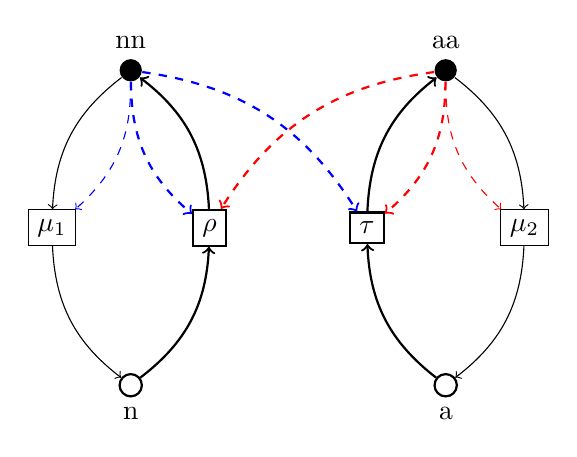
\begin{tikzpicture}

% n node
\node[thick,circle, draw,inner sep=1mm] (n) at (-1,0) {};
\node[below] at (n.south) {n};

% replication reaction node
\node[thick,rectangle,draw] (r) at (0,2) {$\rho$};

% nn node
\node[circle, fill,inner sep=1mm] (nn) at (-1,4) {};
\node[above] at (nn.north) {nn};

\draw[thick,->] (n) to [bend right=25] (r);
\draw[thick,->] (r) to [bend right=25] (nn);

% a node
\node[thick,circle, draw,inner sep=1mm] (a) at (3,0) {};
\node[below] at (a.south) {a};

% translation reaction node
\node[thick,rectangle,draw] (t) at (2,2) {$\tau$};

% nn node
\node[circle, fill,inner sep=1mm] (aa) at (3,4) {};
\node[above] at (aa.north) {aa};

\draw[thick,->] (a) to [bend left=25] (t);
\draw[thick,->] (t) to [bend left=25] (aa);

\draw[thick,dashed,red,->] (aa) to [bend right=25] (r);
\draw[thick,dashed,red,->] (aa) to [bend left=25] (t);
\draw[thick,dashed,blue,->] (nn) to [bend right=25] (r);
\draw[thick,dashed,blue,->] (nn) to [bend left=25]  (t);

% nucleotide degradation reaction node
\node[rectangle,draw] (mun) at (-2,2) {$\mu_1$};

% nucleotide degradation reaction node
\node[rectangle,draw] (mua) at (4,2) {$\mu_2$};

\draw[->] (aa) to [bend left=25] (mua);
\draw[->] (mua) to [bend left=25] (a);

\draw[->] (nn) to [bend right=25] (mun);
\draw[->] (mun) to [bend right=25] (n);

\draw[dashed,red,->] (aa) to [bend right=25] (mua);
\draw[dashed,blue,->] (nn) to [bend left=25] (mun);

\end{tikzpicture}
\end{center}
\caption{\label{fig:simplifiedRAF} A replication-translation RAF. $\{a,n\}$ is the food set. $\{a,n,aa,nn\}$ is the set of species. }
\end{figure}

\section{MASTER representation of full model}

To input our model in MASTER \cite{MASTER} we add indices to represent the sequence and location of each species.  For example, the replication reaction in eq.~\ref{eq:basicRep} is now represented as:

\begin{equation}
 \begin{array}{l l}
 G[i1,i2,i3,l1] + P[a1,a2,a3,l1] + SG[l1]\\
 
\xrightarrow[]{} G[i1,i2,i3,l1] + P[a1,a2,a3,l1] + G[j1,j2,j3,l1],\\
\end{array}
\label{eq:masterRep}
\end{equation}

\noindent{with $i1,i2,i3$ (replicated with some small error to $j1,j2,j3$) denoting the sequence of the species and $l1$ denoting the cell that contains the species.  
Genes occupy space $SG$ within the cell; proteins occupy $SP$.}
The translation reactions in eq.~\ref{eq:basicTrans} are now represented as:

\begin{equation}
 \begin{array}{l l}
G[i1,i2,i3,l1] + P[a1,a2,a3,l1] + SP[l1] \\

\xrightarrow[]{} GP[i1,i2,i3,e1,l1] + P[a1,a2,a3,l1] \\
\\
GP[i1,i2,i3,e1,l1] + P[a1,a2,a3,l1] \\

\xrightarrow[]{} GP1[i1,i2,i3,e1,e2,l1] + P[a1,a2,a3,l1] \\
\\
GP1[i1,i2,i3,e1,e2,l1] + P[a1,a2,a3,l1] \\

\xrightarrow[]{} G[i1,i2,i3,l1] + P[e1,e2,e3,l1] + P[a1,a2,a3,l1] \\
\end{array}
\label{eq:masterTrans}
\end{equation}

\vspace{2mm}
\noindent{with additional indices $e1$ and $e2$ to denote either the `$A$' or `$B$' amino acid forming the partially translated gene-protein complexes $GP$ and $GP1$.}
Each of these reactions has a rate specified within the reaction element.  MASTER also allows the option of applying a rate multiplier, which can be useful for adjusting the rate at which a particular reaction occurs based off of, for example, Hamming distances.
To add a diffusion reaction in MASTER XML a predicate function is used to determine which species will be moved to which location based off of the location indices of the species.  
In the following example, the diffusion space is characterised by an annulus:

\lstset{
  basicstyle=\ttfamily,
  columns=fullflexible,
  showstringspaces=false,
  commentstyle=\color{gray}\upshape
}

\lstdefinelanguage{XML}
{
  morestring=[b]",
  morestring=[s]{>}{<},
  morecomment=[s]{<?}{?>},
  stringstyle=\color{black},
  identifierstyle=\color{darkblue},
  keywordstyle=\color{cyan},
  morekeywords={xmlns,version,type}% list your attributes here
}

\footnotesize{
\begin{lstlisting}

<reaction spec=`Reaction' reactionName="Diffusion_G" rate="0.1">
    <predicate spec=`Predicate' value="abs(l1-l2)==1 || abs(l1-l2)==G_dim[3]"/>
        G[i1,i2,i3,l1] + SG[l2] -> G[i1,i2,i3,l2] + SG[l1]
</reaction>          
        
\end{lstlisting}}

\section{Preliminary simulation results in MASTER}

\normalsize{For the symmetrical monopolymer model, the populations of amino acid and nucleotide food molecules and the `NN' gene and `AA' protein 
quickly reached an equilibrium, as shown in Figure 2.  This also appeared to be true for the `perfect GRT' model (with 3 binary $L=3$ gene species 
and 3 corresponding binary proteins with $L=3$), which behaves as a RAF in that no error is generated by either the replication or translation reactions. 
(In fact, it should be noted that this first implementation of the minimal GRT model in MASTER is actually a CAF, a stronger notion of RAF that has a food 
set - here including genes and proteins along with nucleotides and amino acids - which acts as catalysts immediately in the system). 

However, when only nucleotides and amino acids were initially present in the system (and simulation time was extended), it was observed that one of the 3 gene species quickly stabilized 
while another became predominate and the third went to zero (occasionally being produced in small quantities by random food-generated-only reactions), as shown in Figure 3.

Replacing explicit food molecules (i.e., nucleotide and amino acid species) with spaces - in which the genes occupy a single space $S$, the gene-protein complexes each 
a single space $S$, and the proteins occupy three spaces ($3S$) - caused a similar behaviour but distinctive behaviour.  In this case, one of the 3 gene species clearly began to dominate while 
the other two began to die out and that eventually the whole system collapsed (Figure 4).  Increasing the simulation time again showed that all populations 
clearly went to zero.


\begin{figure}
    \centering
    	\quad
    	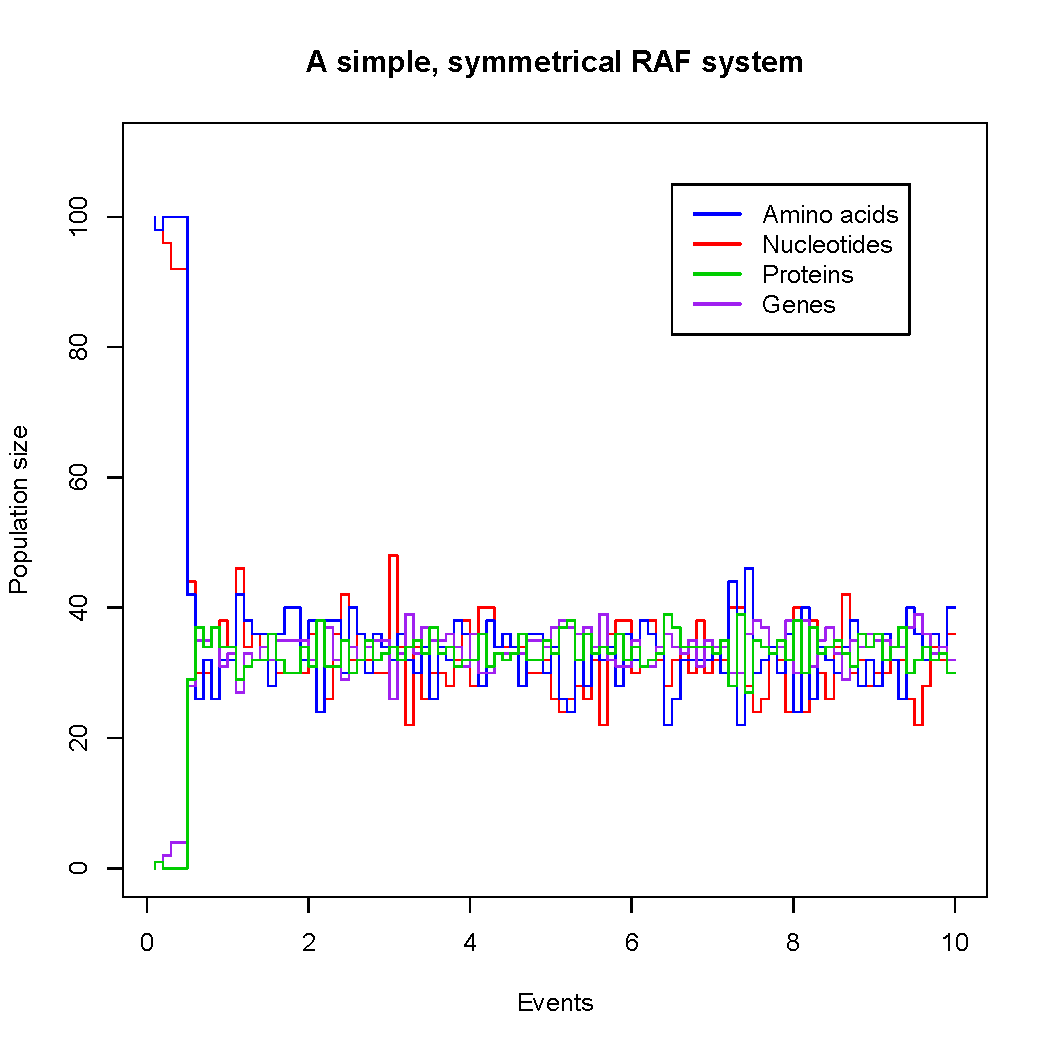
\includegraphics[width=3.5in]{InitiallyOnlyNucAndAAInitiallyUncatalyzed.pdf}
    	\quad
    	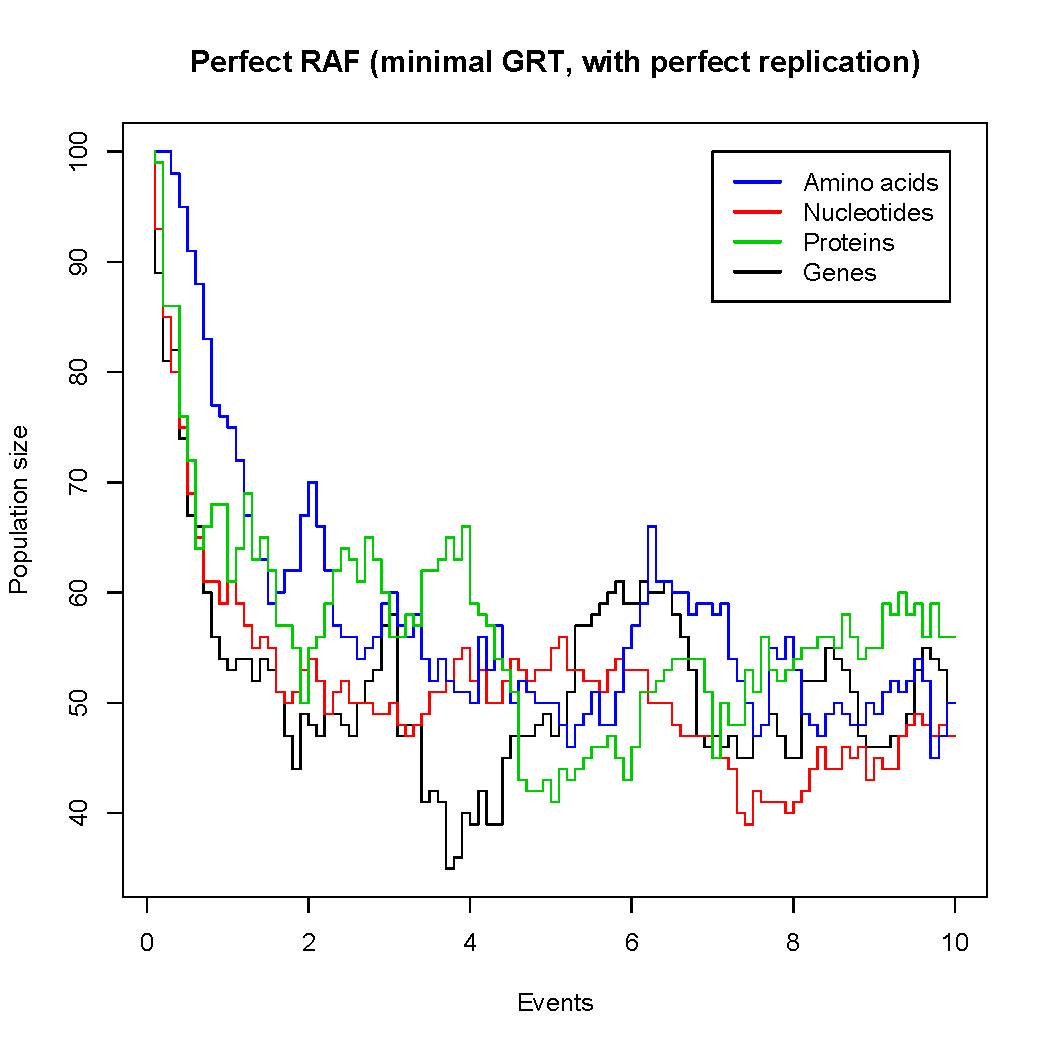
\includegraphics[width=3.5in]{PerfectRAF(minimalGRTnoError).pdf}
    \caption{(top) The simplified monopolymer model with equal initial population sizes for the food set (amino acids and nucleotides).  
    (bottom) The `perfect GRT' model with no reaction errors and with all species present in the initial conditions.}
	\label{fig:monopolymer}
\end{figure}

\begin{figure}
    \centering
    	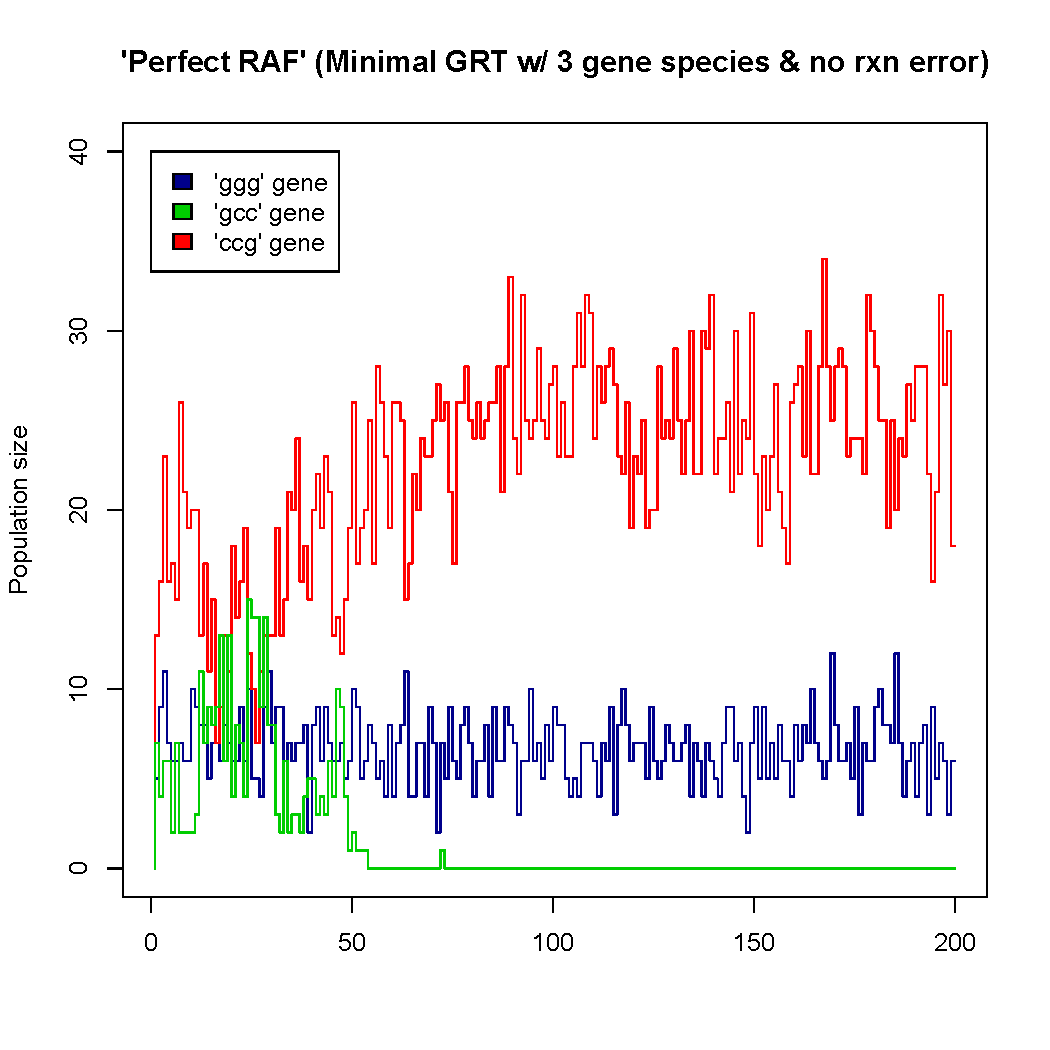
\includegraphics[width=4.5in]{PerfectRAF(minimalGRTnoError)_foodAsSpace(simTime5e4).pdf}
    \caption{The `perfect GRT' model with no reaction errors and with only the food set $F=\{g,c,a,b\}$ as part of the initial conditions, 
    (where $g$ and $c$ are nucleotides and $a$ and $b$ are amino acids).}
	\label{fig:foodAsSpace}
\end{figure}

\begin{figure}
    \centering
    	\quad
    	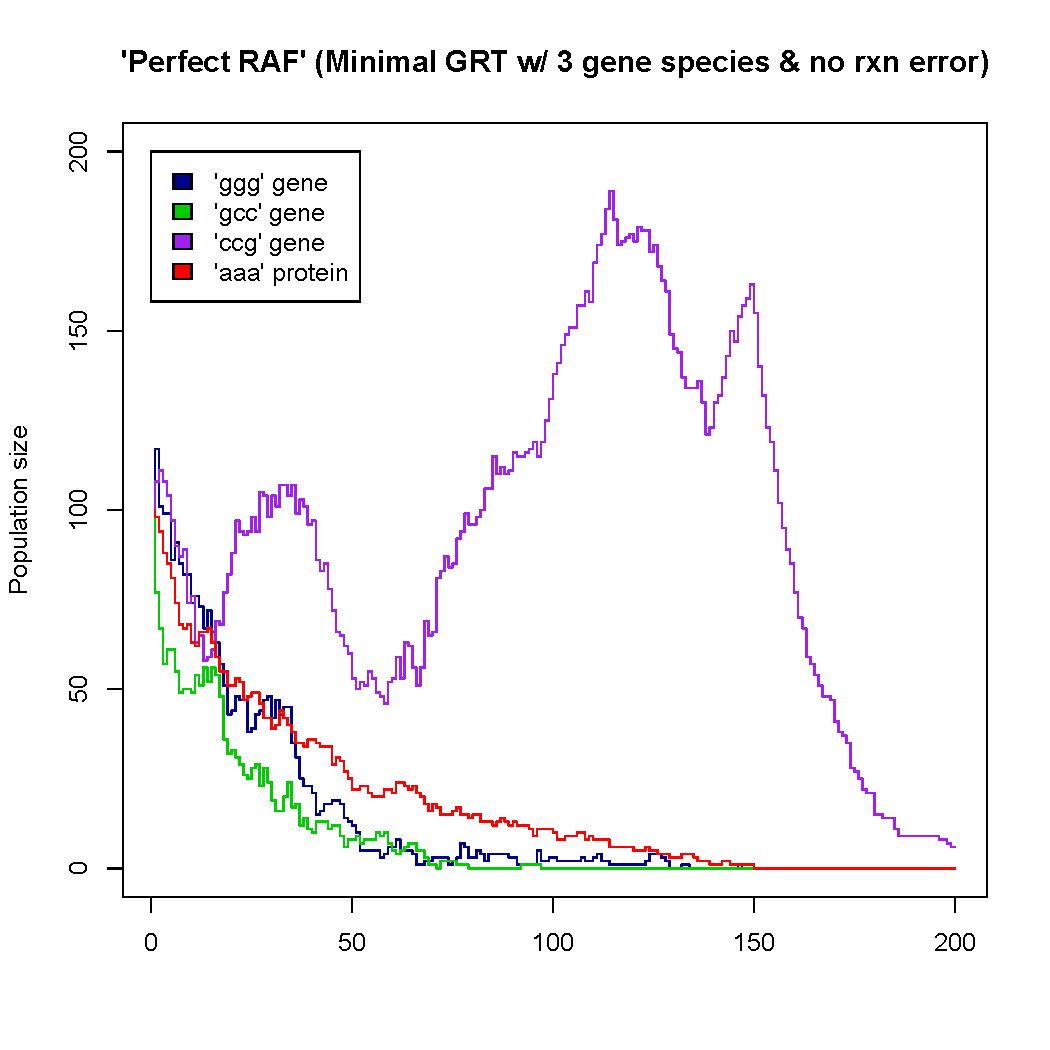
\includegraphics[width=3.5in]{PerfectRAF(minimalGRTnoError)_simTime5e3.pdf}
    	\quad
    	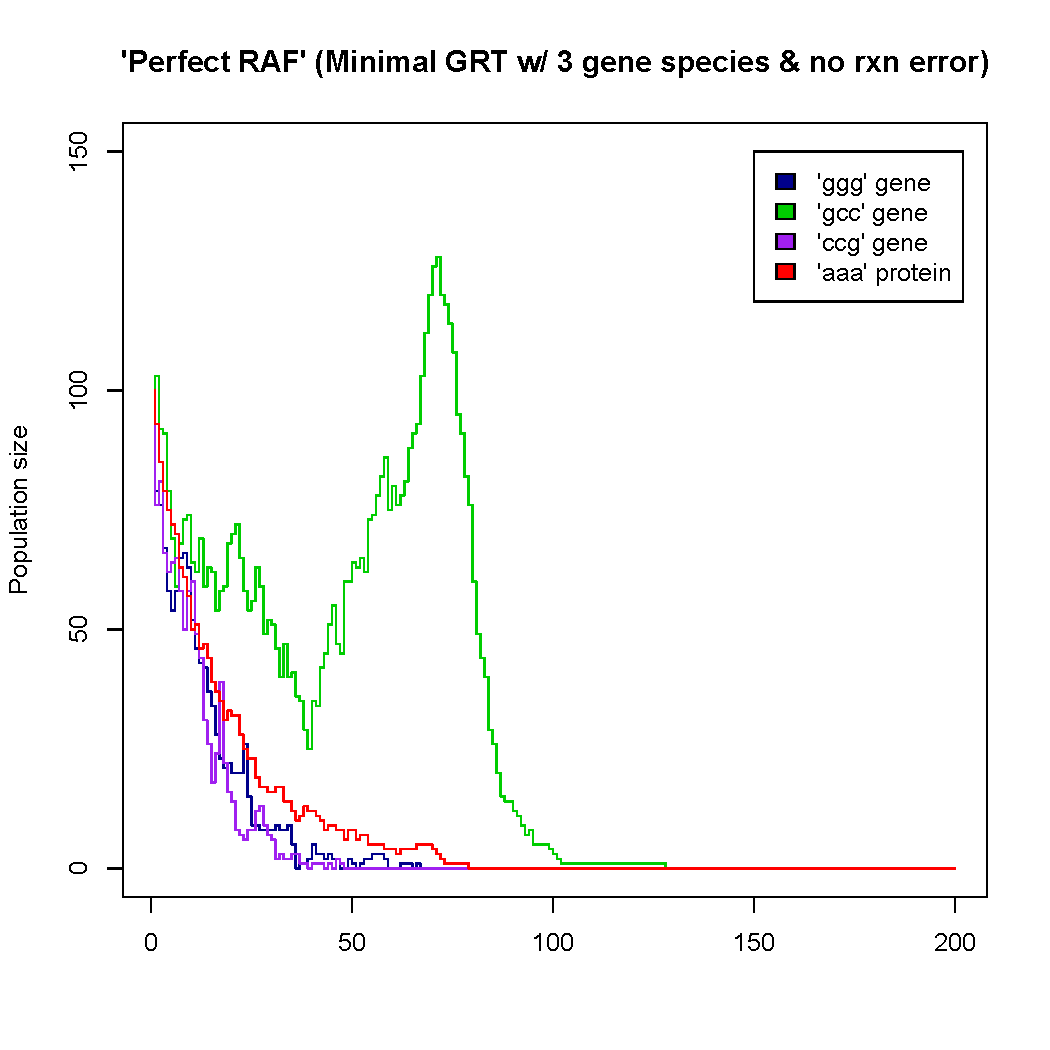
\includegraphics[width=3.5in]{PerfectRAF(minimalGRTnoError)_simTime1e4.pdf}
    \caption{(top) The `perfect GRT' model when the explicit food set was replaced with spaces $S$, with genes occupying $1S$ and proteins occupying $3S$.}
	\label{fig:spaceAsFood}
\end{figure}


%----------------------------------------------------------------------------------------
%	BIBLIOGRAPHY
%----------------------------------------------------------------------------------------
\newpage
\begin{thebibliography}{99} % Bibliography - this is intentionally simple in this template

\bibitem[{{Vaughan and Drummond\/}, 2013}]{MASTER}
{\sc Vaughan, T.~G.} and {\sc A.~J. Drummond}, 2013.
A Stochastic Simulator of Birth–Death Master Equations with Application to Phylodynamics.
\newblock Mol. Biol. Evol.
 
\end{thebibliography}

%----------------------------------------------------------------------------------------
\end{document}